\documentclass{article}
\usepackage{tikz}
\usetikzlibrary{matrix, positioning}

% Define colors
\definecolor{shaded}{RGB}{220,220,220} % Light gray for shaded areas

\begin{document}

\begin{figure}[htbp]
    \centering
    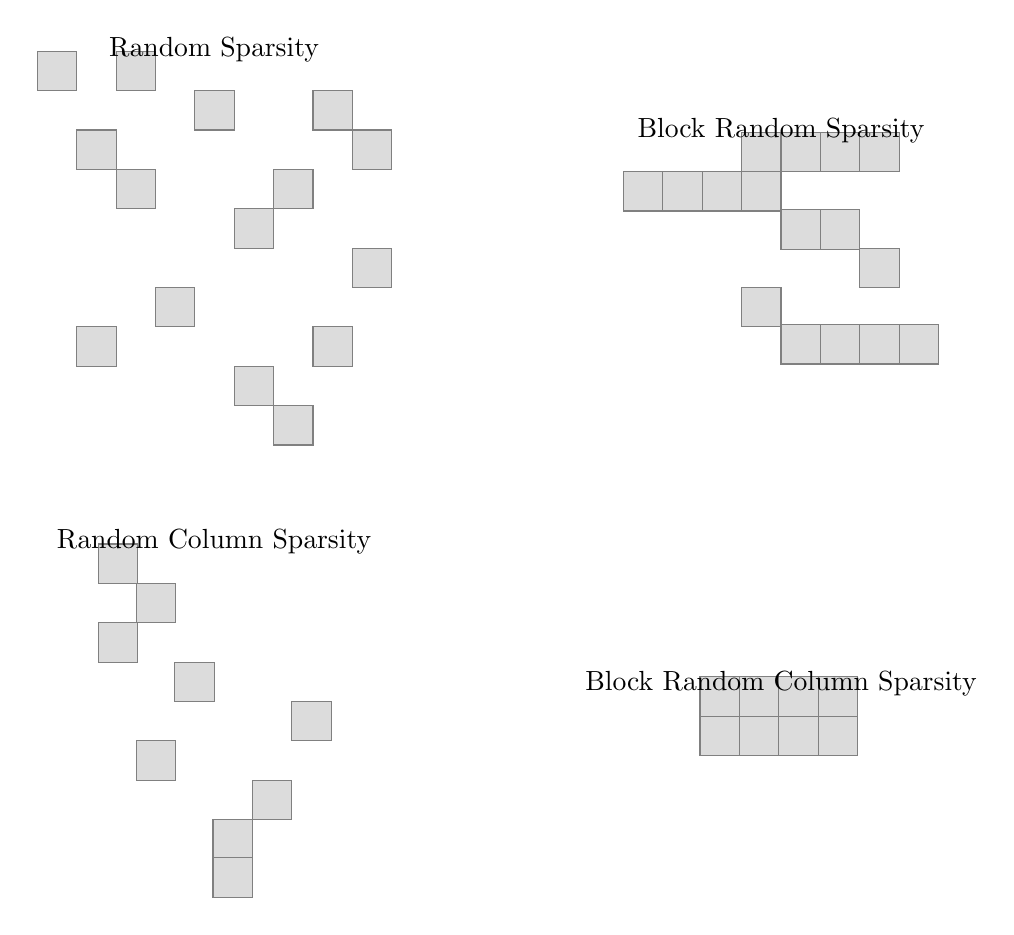
\begin{tikzpicture}[scale=0.6]

    % Style for grids
    \tikzset{
        grid/.style={
            matrix of nodes,
            nodes={
                minimum size=0.5cm,
                anchor=center,
                inner sep=0pt,
                outer sep=0pt,
                draw=black!50,
                fill=white,
                text width=0.48cm,
                align=center,
                font=\scriptsize
            },
            row sep=-\pgflinewidth,
            column sep=-\pgflinewidth
        }
    }

    % Random Sparsity
    \matrix (random) [grid, label={[anchor=north, yshift=0.5em]north:Random Sparsity}] at (0,0) {
        |[fill=shaded]| & & |[fill=shaded]| & & & & & & & \\
        & & & & |[fill=shaded]| & & & |[fill=shaded]| & & \\
        & |[fill=shaded]| & & & & & & & |[fill=shaded]| & \\
        & & |[fill=shaded]| & & & & |[fill=shaded]| & & & \\
        & & & & & |[fill=shaded]| & & & & \\
        & & & & & & & & |[fill=shaded]| & \\
        & & & |[fill=shaded]| & & & & & & \\
        & |[fill=shaded]| & & & & & & |[fill=shaded]| & & \\
        & & & & & |[fill=shaded]| & & & & \\
        & & & & & & |[fill=shaded]| & & & \\
    };

    % Block Random Sparsity
    \matrix (block_random) [grid, label={[anchor=north, yshift=0.5em]north:Block Random Sparsity}] at (12,0) {
        & & & & |[fill=shaded]| & |[fill=shaded]| & |[fill=shaded]| & |[fill=shaded]| & & \\
        & |[fill=shaded]| & |[fill=shaded]| & |[fill=shaded]| & |[fill=shaded]| & & & & & \\
        & & & & & & & & & \\
        & & & & & |[fill=shaded]| & |[fill=shaded]| & & & \\
        & & & & & & & & & \\
        & & & & & & & |[fill=shaded]| & & \\
        & & & & |[fill=shaded]| & & & & & \\
        & & & & & & & & & \\
        & & & & & & & & & \\
        & & & & & |[fill=shaded]| & |[fill=shaded]| & |[fill=shaded]| & |[fill=shaded]| & \\
    };

    % Random Column Sparsity
    \matrix (random_column) [grid, label={[anchor=north, yshift=0.5em]north:Random Column Sparsity}] at (0,-10) {
        |[fill=shaded]| & & & & & & & & & \\
        & & |[fill=shaded]| & & & & & & & \\
        |[fill=shaded]| & & & & & & & & & \\
        & & & & |[fill=shaded]| & & & & & \\
        & & & & & & & & |[fill=shaded]| & \\
        & & |[fill=shaded]| & & & & & & & \\
        & & & & & & & |[fill=shaded]| & & \\
        & & & & & & |[fill=shaded]| & & & \\
        & & & & & & & & & \\
        & & & & & & |[fill=shaded]| & & & \\
    };

    % Block Random Column Sparsity
    \matrix (block_column) [grid, label={[anchor=north, yshift=0.5em]north:Block Random Column Sparsity}] at (12,-10) {
        & & & & & & & & & \\
        & & & & & & & & & \\
        & & & & & & & & & \\
        & & & & & & & & & \\
        & & & & & & & & & \\
        & & & & & & & & & \\
        & & & & & & & & & \\
        & & & & & & & & & \\
        & & & & & |[fill=shaded]| & |[fill=shaded]| & |[fill=shaded]| & |[fill=shaded]| & \\
        & & & & & |[fill=shaded]| & |[fill=shaded]| & |[fill=shaded]| & |[fill=shaded]| & \\
    };

    \end{tikzpicture}
    \caption{Types of sparsity. In random sparsity, any bit may be non-zero. Block-random sparsity assumes aligned, contiguous regions of each row are sparse or not sparse. The degree of block-random sparsity may be lower than the fraction of sparsity when 0s are not fully aligned. We also show random column and random block column sparsity. Block column patterns arise in Deja Vu~\cite{liu2023deja}.}
    \label{fig:sparsity-types}
\end{figure}

\end{document}